We will now consider the symmetries of the LV-model given by
\begin{equation}
  \begin{split}
    \dv{u}{\tau}&=u(1-v),\\
    \dv{v}{\tau}&=\alpha v(u-1).\\    
    \end{split}
  \label{eq:LV}
\end{equation}
Since this model is time-invariant and separable its symmetries are given by
\begin{align}
  X_0&=\partial_\tau+u(1-v)\partial_u+\alpha v(u-1)\partial_v,\label{eq:LV_0}\\
  X_\tau&=\partial_\tau,\label{eq:LV_tau}\\
  X_u&=\dfrac{u}{u-1}\partial_u,\label{eq:LV_u}\\
  X_v&=\dfrac{\alpha v}{1-v}\partial_v.\label{eq:LV_v}
\end{align}
The symmetry of generated by $X_\tau$ in Equation \eqref{eq:LV_tau} corresponds to $\tau$-translations given by
\begin{equation}
\Gamma^{\mathrm{LV},\tau}_{\epsilon}:(\tau,u,v)\mapsto (\tau+\epsilon,u,v).
\end{equation}
For the other two non-trivial generators, i.e. $X_u$ in Equation \eqref{eq:LV_u} and $X_v$ in Equation \eqref{eq:LV_v}, we cannot write down an explicit equation for the symmetry. However, we can write down an implicit expression in terms of their canonical coordinates
\begin{align}
\Gamma^{\mathrm{LV},u}_{\epsilon}:&(s,r_1,r_2)\mapsto(s+\epsilon,r_1,r_2),\quad s=u-\ln(u),r_1=\tau,r_2=v,\label{eq:LV_u}\\
\Gamma^{\mathrm{LV},v}_{\epsilon}:&(s,r_1,r_2)\mapsto(s+\epsilon,r_1,r_2),\quad s=\ln\left(v^{1/\alpha}\right)-\dfrac{v}{\alpha},r_1=\tau,r_2=u.\label{eq:LV_v}\\
\end{align}
In practice, this means that we obtain the transformed coordinates $\hat{u}(\epsilon)$ of $\Gamma^{\mathrm{LV},u}_{\epsilon}$ in Equation \eqref{eq:LV_u} and $\hat{v}(\epsilon)$ of $\Gamma^{\mathrm{LV},v}_{\epsilon}$ in Equation \eqref{eq:LV_v} by solving the following two equations
\begin{align}
u-\ln(u)+\epsilon&=\hat{u}-\ln(\hat{u}),\label{eq:LV_u_implicit}\\
\ln\left(v^{1/\alpha}\right)-\dfrac{v}{\alpha}+\epsilon&=\ln\left(\hat{v}^{1/\alpha}\right)-\dfrac{\hat{v}}{\alpha},\label{eq:LV_v_implicit}
\end{align}
for $\hat{u}$ and $\hat{v}$ respectively. The action of these unidirectional symmetries is illustrated below (Fig \ref{fig:LV_symmetries}). 


\begin{figure}[htbp!]
  \begin{center}
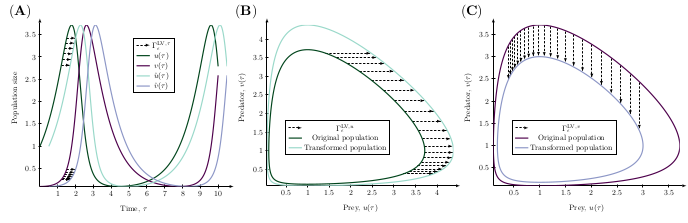
\includegraphics[width=\textwidth]{LV_symmetries}
\caption{\textit{Unidirectional symmetries of the LV-model}. In all cases, the original solution is obtained with the parameter $\alpha=1$, the initial conditions $(u_0,v_0)=(1.00,0.10)$ and the solutions are then transformed with a transformation parameter of $\epsilon=0.5$. (\textbf{A}) The action of the time translation symmetry $\Gamma^{\mathrm{LV},\tau}_{\epsilon}$. (\textbf{B}) The action of the $u$-directional symmetry $\Gamma^{\mathrm{LV},u}_{\epsilon}$. (\textbf{C}) The action of the $v$-directional symmetry $\Gamma^{\mathrm{LV},v}_{\epsilon}$.}
\label{fig:LV_symmetries}
\end{center}
\end{figure}